\documentclass[12pt]{iopart}

\usepackage{hyperref,tikz,array}
\usepackage[export]{adjustbox}
\usepackage{gensymb,eurosym}
\usepackage[numbers]{natbib}
\usepackage[inline]{enumitem}
\usepackage[all]{hypcap}
\pdfminorversion=4
\graphicspath{{Images/}}
\newcolumntype{P}{>{\raggedright\arraybackslash}p}
\usetikzlibrary{arrows.meta, shapes.geometric}
\newcommand{\rpm}{\raisebox{.3ex}{$\scriptstyle\pm$}}
\hypersetup{hidelinks}


\begin{document}
\title[\textit{SI} - Reusing wastewater in agriculture: a Nexus assessment in the NWSAS]{\textit{Supplementary information}\\[12pt] \large Reusing wastewater for agricultural irrigation: a Nexus approach for Sustainable Development in the North Western Sahara Aquifer System}


\author{Camilo Ramirez $^{1}$, Youssef Almulla $^{1}$, and Francesco Fuso-Nerini $^{1}$}

\address{$^{1}$ KTH Royal Institute of Technology, Stockholm, Sweden}
\ead{camilorg@kth.se}
\vspace{10pt}
\begin{indented}
\item[]\today
\end{indented}

\section{Geographic Information Systems analysis}
\begin{table*}[!b]
	\caption{\label{tbl:datasources}Geographic Information System data sources}
	{\footnotesize
		\begin{tabular*}{\textwidth}{@{}P{1.4in} P{1in} l P{1.2in} l l@{}}
			\br
			Layer & Coverage & Format & Resolution & Year & Source\\
			\mr
			Population & Algeria, Tunisia, Libya & raster (tif) & 100 m grid cell & 2015 & \cite{Worldpop2012}\\\ms
			Depth to groundwater & Africa & txt table & 5 km grid cell & 2012 & \cite{Quantitativemapsgroundwater2012a}\\\ms
			Administrative boundaries & Africa & shapefile & Individual country polygons & 2017 & \cite{Humanitarian2017}\\\ms
			Administrative boundaries & Algeria, Tunisia, Libya & shapefile & Level 1 (provinces) polygons & 2015 & \cite{GADM}\\\ms
			Transboundary aquifers borders & Global & shapefile & Individual polygons & 2015 & \cite{IGRAC}\\\ms
			Groundwater quality & NWSAS Basin & data points & 206 data points & 2016 & RA*\\\ms
			Digital Elevation Data* & Africa & raster (tif) & 1, 3 and 15 arc second & 2014 & \cite{DEM2014}\\\ms
			Land cover & Africa & raster (tif) & 20 m grid cell & 2016 & \cite{ESA2017}\\\ms
			Aquifer boundaries & NWSAS basin & shapefile & Individual polygons & - & RA*\\\ms
			Climate data & Global & raster (tif) & 30 arc second, monthly & 1970-2000 & \cite{WorldClimGlobalClimate}\\
			\br
		\end{tabular*}\\
		~* Regional Authorities.
	}
\end{table*}
Geospatial characteristics of the NWSAS were obtained from open sources as described in  \tref{tbl:datasources}. All data layers were converted into matching units, re-projected into the Sud Algerie Degree projection (ESRI: 102592)---This projection was selected as it produces minimal distortions in the analysis area---, re-scaled to the same resolution and, when only individual data points were available, interpolated to extend the data to the entire analysed area (i.e. for the Groundwater quality layer). Furthermore, all layers were merged into a large data frame.

\section{Data calibration}
The \textit{population} and the \textit{irrigated area} layers were calibrated to match regional statistics. The calibration was performed using the fraction given between the regional statistical data (i.e. total population or total irrigated area), and the sum of all data points of the layer in question. The statistical data was available as per country basis. Thus, the calibration process was performed for the basin areas within each country, using their specific information (see \tref{tbl:regionalstats}).

\begin{table*}[!h]
 \caption{\label{tbl:regionalstats}NWSAS population and irrigated area statistics for year 2015, subdivided per country area inside the basin. Data source: \cite{BetterValorizationIrrigation2015}}
 \begin{indented}
 \item[]\begin{tabular}{@{}l*{4}{r}}
 	\br
 	Parameter & Total & Algeria & Tunisia & Libya\\
 	\mr
 	NWSAS Population & 6,376,367 & 4,240,888 & 617,168 & 1,518,311\\
 	NWSAS Irrigated area (Ha) & 469,529 & 237,485 & 56,547 & 175,497\\
 	\br
 \end{tabular}
 \end{indented}
\end{table*}

Moreover, to calibrate the irrigated area data, an algorithm was run to ensure that non of the data cells had more than 100\% of its area covered by irrigated land.

\section{Population and irrigation water withdrawals}
The calculation of total water withdrawals $ww_{tot,i}$ was performed according to \eref{eq:waterwithdrawals}. Population water withdrawals were calculated as the product between the population count in each data cell ($Pop_{i}$) and the specific water demand per capita ($wpc_{i}$) for the region. Similarly, withdrawals from irrigated agriculture were calculated as the product between the irrigated area inside each data cell ($IrrArea_{i}$) and the specific water demand per cultivated hectare ($wpha_{i}$) for the region.

\begin{equation}\label{eq:waterwithdrawals} 
 ww_{tot,i} = Pop_{i}\cdot wpc_{i} +IrrArea_{i}\cdot wpha_{i} 
\end{equation}

For the baseline, a level of water withdrawals per capita $wpc$ of 55 cubic meters per year was assumed with a population growth of 1\% per year \cite{Householdwaterconsumption2014}. Moreover, all cropland area within the aquifer was considered to be irrigated by groundwater resources and the water requirements per cultivated hectare $wpha$ to be 13,520 m\textsuperscript{3}/Ha for the Algerian part; 13,266 m\textsuperscript{3}/Ha for Tunisia and 9,134 m\textsuperscript{3}/Ha for Libya, according to data from \cite{Socioeconomicaspectsirrigation2014}. Finally, no growth in irrigated area was considered.

\section{Groundwater pumping}\label{Sc:pumping}
The energy needs to pump water from groundwater resources is given by the required lift ($H-h$), the pressure drop due to fluid friction in the piping, and the pressure losses in valves and fittings. Pressure losses due to friction in the piping were found to be rather small compared to the lift requirements. Therefore, and due to lack of specific data on wells and boreholes in the region, the pressure losses due to friction in the piping and in valves and fittings were disregarded. The energy requirements (in watt-h) can then be estimated as \eref{eq:1} \cite{Groundwaterdependentirrigationcosts2017}:

\begin{equation}\label{eq:1}
E = \frac{Q\cdot(\rho\cdot g\cdot(H - h))}{\eta}
\end{equation}

Where $Q$ stands for the water extractions (m\textsuperscript{3}), $\rho$ for the water density (kg/m\textsuperscript{3}), $g$ for the gravitational acceleration (m/s\textsuperscript{2}), $H$ for the delivered hydraulic head (meters), and $h$ for the head in the well (meters). Moreover, $\eta$ accounts for the pumping efficiency, which was set as 85\% along the entire aquifer.

\section{Wastewater Treatment System characteristics}
FAO standards for population wastewater pollutant levels and reused water quality for agricultural irrigation \cite{fao1985water}, were used for the entire NWSAS area. These are shown in \tref{tbl:pollutans}.

\begin{table*}[!ht]
	\caption{\label{tbl:pollutans}Pollutant levels of wastewater and treated wastewater (mg/l).}
	\begin{indented}
	\item[]\begin{tabular}{@{}l r r}
		\br
		Pollutant type & Wastewater & Treated wastewater\\
		\mr
		Suspended solids ($SS$) & 900 & 100\\
		Nitrogen ($N$) & 40 & 10\\
		Phosphorus ($P$) & 20 & 2\\
		Biochemical Oxygen Demand (BOD\textsubscript{5}) ($BOD_5$) & 500 & 50\\
		Chemical Oxygen Demand ($COD$)& 500 & 50\\
		\br
	\end{tabular}
	\end{indented}
\end{table*}

Cost functions for different WWTT taken from the work of \citet{Assessmentwastewatertreatment2012}, were used to evaluate the competence of selected technologies in the NWSAS. Energy intensity characteristics were added for each technology according to \cite{Energypatternanalysis2012,ComparativeAnalysisEnergy2017}. The characteristics of the different WWTT and their cost and energy functions are presented in \tref{tbl:treatmentsystems}.

\begin{table*}[!h]
    \caption{\label{tbl:treatmentsystems}Treatment systems analyzed Adapted from \cite{Assessmentwastewatertreatment2012}, Copyright (2012), with permission from Elsevier.}
    \addtocounter{table}{-1}
\end{table*}
	~\\[-50pt]{\footnotesize
	\begin{longtable}{@{}P{1.2in} P{0.9in} P{1.9in} P{0.7in} P{0.7in}}
	\br
    Technology & Pollutant removal (\%) & Costs (\euro) & Energy (kWh)$^{\dagger}$ & Usage\\
    \mr
    \endfirsthead
    \multicolumn{4}{@{}l}{\ldots continued}\\\br
    Technology & Pollutant removal (\%) & Costs (\euro) & Energy (kWh)$^{\dagger}$ & Usage\\\mr
    \endhead % all the lines above this will be repeated on every page
    \br
    \multicolumn{4}{r@{}}{continued \ldots}\\
    \endfoot
    \endlastfoot
    Pond System (PS) & N: 20 -- 40 \newline P: 60 -- 70 \newline COD: 60 -- 96 \newline SS: 50 -- 90 & CAPEX: $3897.7\cdot x^{-0.407}$ \newline OPEX: $5.543\cdot x + 3127.5$ & $0.19\cdot V$ & Irrigation tailwater\\
    Intermittent Sand Filter (ISF) & N: 65 -- 95 \newline P: 75 -- 99 \newline COD: 75 -- 90 \newline SS: 85 -- 95 & CAPEX: $2115.5\cdot x^{-0.399}$ \newline OPEX: $12.026\cdot x+3518.9$ & $0.2\cdot V$ & Domestic wastewater\\
    Trickling Filter (TF) & N: 35 -- 50 \newline P: 35 -- 55 \newline COD: 75 -- 90 \newline SS: 50 -- 90 & CAPEX: $12237\cdot x^{-0.87}$ \newline OPEX: $13.504\cdot x+6020$ & $0.3\cdot V$ & Domestic wastewater\\
    Moving Bed Biofilm Reactor (MBBR) & N: 10 -- 20 \newline P: 30 -- 40 \newline COD: 20 -- 40 \newline SS: 60 -- 80 & CAPEX: $1187\cdot x^{-0.165}$ \newline OPEX: $12.794\cdot x+6031$ & $0.8\cdot V$ & Domestic wastewater\\
    Rotating Biological Contractors (RBC) & N: 20 -- 80 \newline P: 10 -- 30 \newline COD: 70 -- 93 \newline SS: 75 -- 98 & CAPEX: $6931.4\cdot x^{-0.383}$ \newline OPEX: $313.4\cdot x^{-0.435}$ & $0.8\cdot V$ & Domestic wastewater\\
    Membrane Bioreactor (MBR) & N: 50 -- 90 \newline P: 20 -- 70 \newline COD: 70 -- 90 \newline SS: 85 -- 99 & CAPEX: $5635.3\cdot x^{-0.352}$\newline $^{*}$OPEX: $2.116\cdot V^{0.713}e^{1.51\cdot SS+0.037\cdot BOD}$ & $0.8\cdot V$ & Domestic wastewater\\
    Extended Aeration (EA) & N: 50 -- 90 \newline P: 15 -- 70 \newline COD: 70 -- 90 \newline SS: 85 -- 99 & CAPEX: $7946\cdot x^{-0.460}$ \newline $^{*}$OPEX: $169.48\cdot V^{0.454}e^{0.61\cdot SS}$ & $0.6\cdot V$ & Domestic wastewater\\
    Sequencing Batch Reactor (SBR) & N: 55 -- 90 \newline P: 25 -- 70 \newline COD: 70 -- 90 \newline SS: 85 -- 99 & CAPEX: $8258.9\cdot x^{-0.407}$ \newline OPEX: $309.4\cdot x^{-0.389}$ & $1\cdot V$ & Domestic wastewater\\
    \br
    \multicolumn{4}{@{}l}{$x$: population equivalent, $x=V\times1500/(400\times365)$, $V$: wastewater flow (m\textsuperscript{3}/yr)} \\
    \multicolumn{4}{@{}l}{N: Nitrogen, P: Phosphorus, COD: Chemical Oxygen Demand, SS: Suspended Solids} \\
    \multicolumn{4}{@{}l}{CAPEX: Capital Expenditure, OPEX: Operating Expenses}\\
    $^{*}$ Taken from \cite{Costmodellingwastewater2011} & & & \\ 
    $^{\dagger}$ Based on \cite{Energyrequirementswater2012,ComparativeAnalysisEnergy2017} & & & 
    \end{longtable}
	}

\section{Reverse Osmosis desalination}\label{Sc:RO}
Reverse Osmosis (RO) desalination is the most popular desalination technology used worldwide. Its energy intensity falls typically in the range of 0.5 to 2.5 kWh per cubic meter of desalinated brackish water \cite{Energyoptimalgroundwater2013}.

To estimate the energy required to desalinate one cubic meter of saline water, often detailed information of the RO system is required. When analysing a broad area using a geospatial approach, such information is not available as the characteristics of the system can change from application to application \cite{stillwellPredictingSpecificEnergy2016,aminfardMultilayeredSpatialMethodology2019}. Thus, a simplified approach was used to estimate the RO energy requirements. RO is a pressure-driven process that forces water through a membrane which separates dissolved solutes using preferential diffusion. The output water from the membrane (\textit{permeate, p}) is relatively free of solutes, while the remaining water (\textit{concentrate, c}) exits the pressure vessel with a high concentration of solutes (i.e. high TDS levels). A schematic representation of the process is presented in \fref{fig:ro} \cite{crittenden_mwhs_2012}.

\begin{figure}[!h]
	\centering
	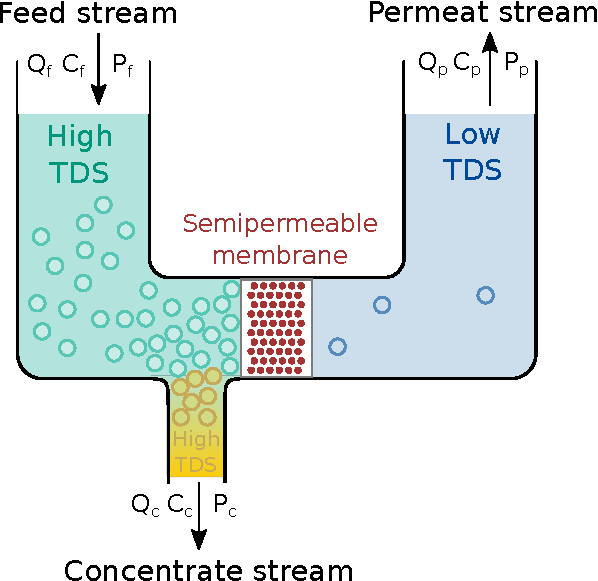
\includegraphics[width=0.4\textwidth]{Reverse_Osmosis}
	\caption[Reverse Osmosis schematic separation process]{Reverse osmosis schematic separation process. Based on: \cite{crittenden_mwhs_2012}.}
	\label{fig:ro}
\end{figure} 

The minimum energy required to push the water through the membrane is given by the amount of diluted solutes in the \textit{feed (f)} water. Such minimum energy can be estimated calculating the osmotic pressure of the \textit{feed} water, as described in \eref{eq:6} \cite{crittenden_mwhs_2012}.

\begin{equation}\label{eq:6}
\pi = \phi\cdot C\cdot R\cdot T
\end{equation}

\noindent{Where}:
\begin{itemize}[label={-}]
	\item $\pi$: osmotic pressure (bar),
	\item $\phi$: osmotic coefficient, close to 1 (-), assumed a 0.95 \cite{crittenden_mwhs_2012},
	\item $C$: concentration of all solutes (mol/L),
	\item $R$: universal gas constant, 0.083145 (L$\cdot$bar/mol$\cdot$K),
	\item $T$: absolute temperature (K), (273 + \degree C), assumed at 25 \degree C for the entire aquifer.
\end{itemize}~

Thus, the minimum energy demand can be estimated multiplying the osmotic pressure of the \textit{feed} water $\pi$ (in bar) by a conversion factor of 1.0 kWh/m\textsuperscript{3} = 36 bar. In reality, the energy demanded is greater due to factors as friction losses, membrane filtration resistance, among others. However, this approach has been used in cases were no specific data of the RO system is available \cite{KARABELAS201815}.

The water quality layer used, was obtained from 206 measurements provided by National Authorities of the region. Each point specifies the spacial location and groundwater TDS content. Although the data did not covered the entire basin area, due to lack of any other related information it was used to produced a raster layer. An inverse distance weighted interpolation method, having as distance weighting factor an inverse distance to a power of 2 and a global search radius with maximum number of nearest points of 10 was used (see \fref{fig:TDS}).

\begin{figure*}[!h]
	\centering
	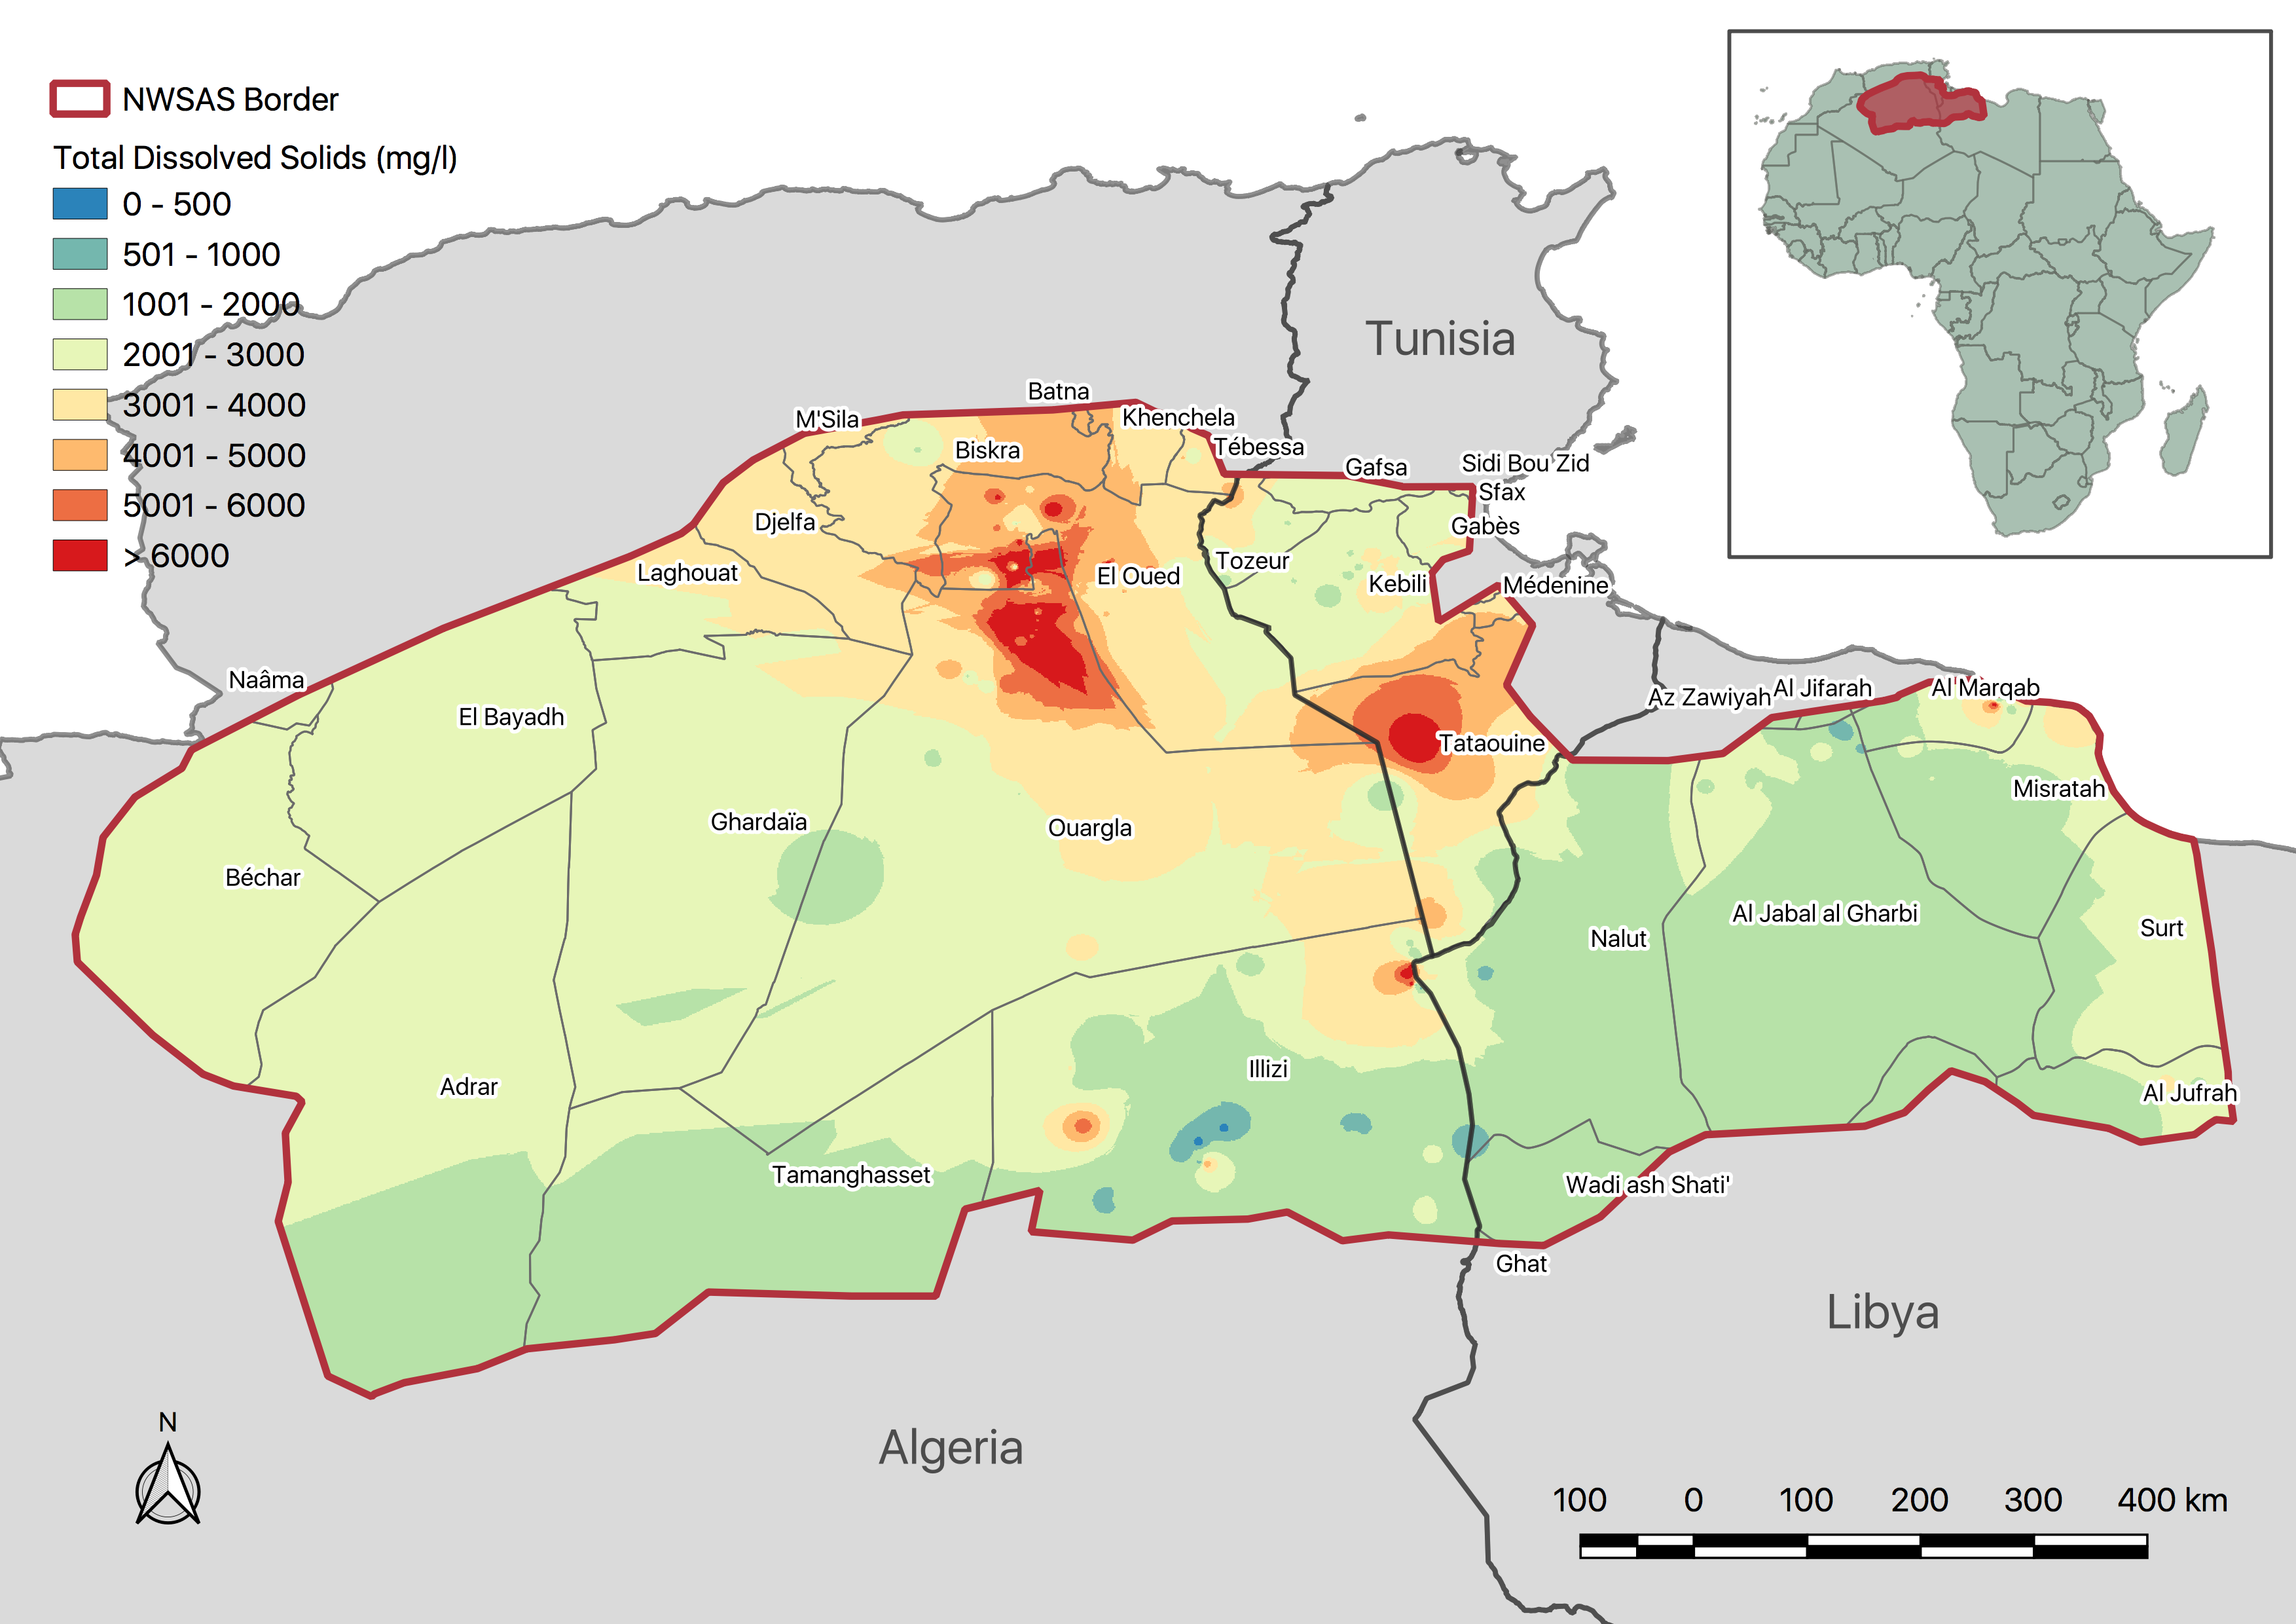
\includegraphics[width=0.88\textwidth, cfbox=black 1pt 0pt]{NWSAS_TDS}
	\caption[NWSAS groundwater quality map - Total Dissolved Solids (TDS)]{North Western Sahara Aquifer System - Groundwater quality map, Total Dissolved Solids (TDS) at 1$\times$1 km grid cell resolution.}
	\label{fig:TDS}
\end{figure*}

\section{Energy-for-wastewater}\label{Sc:eww}
To calculate the energy-for-wastewater requirements an energy intensity factor was used for each evaluated treatment technology following \eref{eq:energy-for-wastewater}.

\begin{equation}\label{eq:energy-for-wastewater}
E_{ww} = Q_{ww,yr}\cdot X_t
\end{equation}

Where $Q_{ww,yr}$ represents the yearly treated wastewater in m\textsuperscript{3}/yr, and $X_t$ the average energy demand of the specific WWTT $t$, to treat one m\textsuperscript{3} of wastewater (in kWh/m\textsuperscript{3}).

\newcommand{\newblock}{}
\bibliography{References}
\bibliographystyle{unsrtnat}

\end{document}